\section{Speculative Transformer search}
\label{sec:search}

\subsection{Exact parents and long-prefix failure}

On the held-out CUDA run, repeated evaluations of the midpoint
force agreed byte for byte, and the tangent calculation passed
its finite-difference check. Both integer formats recovered
position and momentum at all \PthreeParents{} checked tree
parents. Neither lost an entire nonzero shear on those traversals.
Intended-rule token accuracy and solve rate met both pre-specified
fidelity criteria. Native replay returned with nonzero tree
errors. The integer inverse reconstructs the realized lattice
trajectory exactly even when the rounded forward update differs
from the native binary32 step.

The long lattice tape used seed \PthreeLongSeed{} at
\(h=\PthreeLongStep{}\), with position and momentum shifts
\PthreeIntLowShifts{} for int32 and \PthreeIntHighShifts{} for
int64. Int32 reached its state-range guard at step
\PthreeIntLowGuard{}, and int64 reached its conservative guard
for exact intermediate arithmetic at step \PthreeIntHighGuard{}.
Neither run met the long-tape criterion, although their final
completed prefixes, at \PthreeIntLowPrefix{} and
\PthreeIntHighPrefix{} steps, rewound exactly. The first nonzero
kicks that rounded away entirely occurred at
steps \PthreeIntLowKick{} and \PthreeIntHighKick{}, respectively.
We varied \(h\) on separate native trajectories. At
\(h=\PthreeHighStep{}\), both trajectories crossed the relative
error tolerance \PthreeNativeThreshold{} earlier than their
smaller-step counterparts. For each trajectory, we fit both
models to the same observations with
\(0<\rho_T<\PthreeFitErrorUpper{}\). At the larger step size,
each seed had \PthreeHighFitN{} eligible observations at
\(T\in\{\PthreeHighFitSteps{}\}\), and the power law fit better
than the corresponding exponential in both cases. P3-A therefore
failed its long-tape and native-growth criteria despite passing
the parent reconstruction and forward-fidelity checks.

\begin{table}[tbp]
  \centering\small
  \caption{Phase~3 native directional stretch and growth fits.
  Threshold crossings are on the registered sampled grid. The
  directional rate uses the reported endpoint \(T=\PthreeRateHorizon{}\).
  The fit sample count includes only errors with
  \(0<\rho_T<\PthreeFitErrorUpper{}\), used by both models.}
  \label{tab:transformer}
  % Generated by scripts/build_tables.py
% Source: artifacts/sol/p3/sol-20261122-cuda-lock/test_parts/physics.json physics.native_runs[*].{fit,samples[-1]}
\begin{tabular}{@{}rrrrrrr@{}}
\toprule
Seed & $h$ & First miss & Fit $n$ & $G_{500}/(500h)$ & Exp. $R^2$ & Power $R^2$ \\
\midrule
\ensuremath{57037} & \ensuremath{1/32} & \ensuremath{256} & \ensuremath{7} & \ensuremath{0.713} & \ensuremath{0.978} & \ensuremath{0.879} \\
\ensuremath{57037} & \ensuremath{1/16} & \ensuremath{128} & \ensuremath{5} & \ensuremath{2.776} & \ensuremath{0.935} & \ensuremath{0.987} \\
\ensuremath{57037} & \ensuremath{1/8} & \ensuremath{32} & \ensuremath{4} & \ensuremath{3.525} & \ensuremath{0.798} & \ensuremath{0.962} \\
\ensuremath{57119} & \ensuremath{1/32} & \ensuremath{128} & \ensuremath{6} & \ensuremath{2.286} & \ensuremath{0.958} & \ensuremath{0.863} \\
\ensuremath{57119} & \ensuremath{1/16} & \ensuremath{128} & \ensuremath{5} & \ensuremath{9.219} & \ensuremath{0.945} & \ensuremath{0.893} \\
\ensuremath{57119} & \ensuremath{1/8} & \ensuremath{32} & \ensuremath{4} & \ensuremath{1.011} & \ensuremath{0.951} & \ensuremath{0.970} \\
\bottomrule
\end{tabular}

\end{table}

\subsection{Branching utility and detectable preference}

At depth \PthreeDepth{}, each reversible format solved all
\PthreeDfsSolved{} admissible rules per public seed, while the
single path solved \PthreeSingleSolved{}. Rules that differ at
an address require incompatible predictions there, so a single
submission succeeds with probability at most \(1/(D+1)\) under
the uniform prior. The single-path control attained that bound.
Depth-first search improved exact-prior and sampled coverage at
every tested depth by allowing additional terminal submissions.
We compute exact-prior coverage by enumerating the \(D+1\) rules
for each of \PthreeSeeds{} public models. Sampled coverage uses
\PthreeDrawsPerSeed{} private draws per model, or
\PthreeSingleSampledCases{} total. At depth \PthreeDepth{},
the single path solved
\PthreeSingleExactSolved{}/\PthreeSingleExactCases{} exact-prior cases
and \PthreeSingleSampledSolved{}/\PthreeSingleSampledCases{} sampled
draws. Private draws on the same model share its trajectory.
The public model seed is the unit of replication.

P3-B also required smooth probe-loss trajectories in both
outcome classes and low orientation-free ROC--AUC for a
pre-specified detector bank that included a fitted ridge score.
Both conditions held, with a maximum gated AUC of \PthreeAuc{}
across the registered depths. We evaluated discrimination on
the first leaf and used pair weighting to compare surviving
histories within later visit ranks. Conditioning on rank matters
because earlier failures change the remaining distribution of
private rules.

\begin{table}[tbp]
  \centering\small
  \caption{Confirmatory coverage counts and detector maxima by search depth.
  Exact prior enumerates \PthreeSeeds{} public models times \(D+1\)
  rules. Sampled uses \PthreeDrawsPerSeed{} draws per public model.
  All three DKD formats have the same coverage. Gated AUC is the maximum
  across the pre-specified signal banks and formats. Rank AUC uses visit
  rank alone on histories still alive after earlier failures.}
  \label{tab:branching}
  % Generated by scripts/build_tables.py
% Source: artifacts/sol/p3/sol-20261122-cuda-lock/test.json decisions.depths[*].{methods,monitors}
% Source: artifacts/sol/p3/sol-20261122-cuda-lock/test_parts/{native,int32,int64,single}_*.json cell.rows[*].{leaves,private_draws}
\begin{tabular}{@{}rrrrrrr@{}}
\toprule
Depth & DFS exact & Single exact & DFS sampled & Single sampled & Gated AUC & Rank AUC \\
\midrule
\ensuremath{1} & \ensuremath{6/6} & \ensuremath{3/6} & \ensuremath{384/384} & \ensuremath{192/384} & \ensuremath{0.554} & \ensuremath{0.750} \\
\ensuremath{2} & \ensuremath{9/9} & \ensuremath{3/9} & \ensuremath{384/384} & \ensuremath{130/384} & \ensuremath{0.513} & \ensuremath{0.719} \\
\ensuremath{4} & \ensuremath{15/15} & \ensuremath{3/15} & \ensuremath{384/384} & \ensuremath{70/384} & \ensuremath{0.547} & \ensuremath{0.712} \\
\ensuremath{8} & \ensuremath{27/27} & \ensuremath{3/27} & \ensuremath{384/384} & \ensuremath{46/384} & \ensuremath{0.536} & \ensuremath{0.683} \\
\bottomrule
\end{tabular}

\end{table}

Batched arithmetic assigned slightly different ridge scores to
identical feature rows. In a post-hoc check, we scored each
unique row once and assigned that score to every corresponding
private draw. Under the exact prior, each leaf wins for exactly
one rule, so a deterministic score with no access to the private
rule has the same distribution in both outcome classes. The
tie-safe calculation gave the expected chance AUC. The confirmatory
decision uses the pre-specified calculation and applies to the
tested signals, task, and information set.

\subsection{Dense checkpoints, offload, and a smaller trainable state}

P3-C met the pre-specified requirements for allocation, solve
rate, and native forward speed. At the larger tested depths,
all reversible formats used less allocated GPU memory than both
dense resident checkpoint baselines. At depth \PthreeDepth{},
int32 used \PthreeIntLowMiB{} MiB, compared with
\PthreeGpuSgdMiB{} MiB for GPU-checkpoint SGD. In the held-out
run, native DKD forward blocks took \PthreeNativeRatio{} times
the SGD forward time. Traversal also involves work beyond the
forward gradient budget, including force recomputation in rewind
and the range checks and state conversions of the integer formats.

With pinned checkpoints, SGD moves the saved state over PCIe
without another gradient evaluation. An int32 rewind step instead
recomputes the midpoint force and performs the fixed-point state
updates. At this model size, a complete pinned SGD state round
trip took \PthreeSgdRoundTrip{} ms and one int32 reverse step
took \PthreeIntLowRewind{} ms. Rewind already cost more than
copying at the shortest tested suffix for all reversible formats,
both pinned baselines, and both restore-only and round-trip
accounting. At the same depth and solve rate, pinned-host SGD
used \PthreePinnedSgdMiB{} MiB on the GPU and exhausted the tree
in \PthreePinnedSgdSeconds{} s, compared with
\PthreeIntLowSeconds{} s for int32. This
\PthreePinnedSpeedup{}\(\times\) speedup came with a larger
host working set.

\begin{table}[tbp]
  \centering\small
  \caption{Measured resource use at search depth \PthreeDepth{}.
  The exact and sampled columns count the cohorts in
  Table~\ref{tab:branching}. Memory peaks are maxima over public
  model seeds. Exhaustion time is a median. Mean stopping time
  includes all sampled private draws, charging full exhaustion
  on failures. The exploratory head-only control uses the same
  test seeds and a smaller trainable subset.}
  \label{tab:systems}
  % Generated by scripts/build_tables.py
% Source: artifacts/sol/p3/sol-20261122-cuda-lock/test.json decisions.depths.8.methods
% Source: theory/evidence/phase3/sol_replication_audit.json P3_C.cells and head_only_control
% Source: artifacts/sol/p3/sol-20261122-cuda-lock/test_parts/*_8.json and theory/evidence/phase3/sol_head_control.json cell.rows[*].{leaves,private_draws,elapsed}
\begin{tabular}{@{}lrrrrrr@{}}
\toprule
Method & Exact & Sampled & GPU MiB & Host GiB & Exhaust s & Stop s \\
\midrule
Native DKD & \ensuremath{27/27} & \ensuremath{384/384} & \ensuremath{264.7} & \ensuremath{1.62} & \ensuremath{1.432} & \ensuremath{0.655} \\
Int32 DKD & \ensuremath{27/27} & \ensuremath{384/384} & \ensuremath{305.8} & \ensuremath{1.71} & \ensuremath{2.370} & \ensuremath{1.029} \\
Int64 DKD & \ensuremath{27/27} & \ensuremath{384/384} & \ensuremath{457.2} & \ensuremath{1.71} & \ensuremath{2.461} & \ensuremath{1.076} \\
Momentum SGD, GPU & \ensuremath{27/27} & \ensuremath{384/384} & \ensuremath{906.6} & \ensuremath{1.62} & \ensuremath{1.028} & \ensuremath{0.505} \\
AdamW, GPU & \ensuremath{25/27} & \ensuremath{357/384} & \ensuremath{1388.1} & \ensuremath{1.66} & \ensuremath{1.008} & \ensuremath{0.564} \\
Momentum SGD, pinned & \ensuremath{27/27} & \ensuremath{384/384} & \ensuremath{264.7} & \ensuremath{2.62} & \ensuremath{1.028} & \ensuremath{0.549} \\
AdamW, pinned & \ensuremath{25/27} & \ensuremath{357/384} & \ensuremath{425.2} & \ensuremath{3.16} & \ensuremath{1.090} & \ensuremath{0.676} \\
Single path & \ensuremath{3/27} & \ensuremath{46/384} & \ensuremath{264.7} & \ensuremath{1.62} & \ensuremath{0.191} & \ensuremath{0.213} \\
\midrule
\multicolumn{7}{@{}l@{}}{\textit{Exploratory head-only control on reused seeds}} \\
Momentum SGD, GPU & \PthreeHeadSolved/\PthreeHeadCases & \PthreeHeadSampledSolved/\PthreeHeadSampledCases & \PthreeHeadMiB & \ensuremath{1.62} & \PthreeHeadSeconds & \PthreeHeadStopSeconds \\
\bottomrule
\end{tabular}

\end{table}

\begin{figure}[tbp]
  \centering
  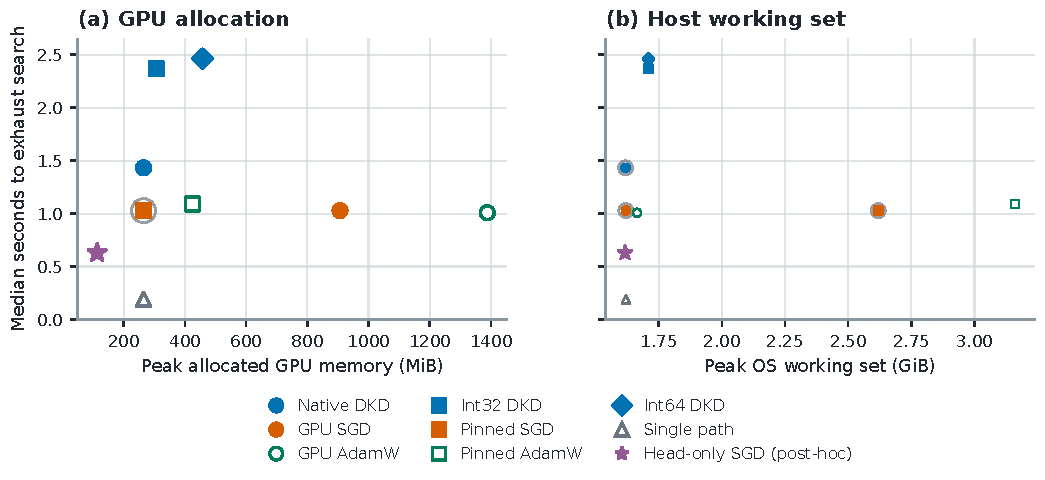
\includegraphics[width=\linewidth]{figures/fig3_systems_pareto.pdf}
  \caption{Measured depth-\PthreeDepth{} search resource tradeoff.
  Exhaustive elapsed time is paired with peak allocated GPU memory
  and peak host working set. Hollow marks indicate incomplete exact-prior
  coverage. Rings identify nondominated confirmatory full-coverage methods in
  each projection. The star marks the exploratory head-only control.}
  \label{fig:systems}
\end{figure}

\paragraph{Exploratory output-head control.}
To test whether the task required full-backbone adaptation, we
ran an exploratory control with the backbone frozen. We trained
the \PthreeHeadParams{} coordinates of the existing output
matrix with momentum SGD and reused the support batches,
verifier, and unresolved-fork policy. On the previously scored
seeds, the head alone solved
\PthreeHeadSolved{}/\PthreeHeadCases{} model-rule pairs. Peak
GPU allocation was \PthreeHeadMiB{} MiB, with at most
\PthreeHeadKiB{} KiB in live head checkpoints. Mean sampled
stopping time was \PthreeHeadStopSeconds{} s. The control
changes both checkpoint size and backward work. It shows that
head-only adaptation sufficed on this search task. The
confirmatory memory comparison concerns full-model adaptation.
